\documentclass[12pt,journal,draftcls,letterpaper,onecolumn]{IEEEtran}
\makeatletter
\usepackage{cite}
\usepackage{amssymb}
\usepackage{amsmath}
\usepackage{graphicx}
%\usepackage[retainorgcmds]{IEEEtrantools}
%\usepackage{algorithm}
%\usepackage{algorithmic}
%\usepackage{subfigure}
%\usepackage{url}
\begin{document}
\title{Evolution of Free-riding in P2P Networks}
\author{\IEEEauthorblockN{Heungsik Eom}\\
\IEEEauthorblockA{Electrical and Computer Engineering\\
University of Florida\\
Gainsville, Florida 32611\\
Email: eomhes@gmail.com}\\
\and
\IEEEauthorblockN{P. Oscar Boykin}\\
\IEEEauthorblockA{Electrical and Computer Engineering\\
University of Florida\\
Gainsville, Florida 32611\\
Email: boykin@acis.ufl.edu}
}
\maketitle

\begin{abstract}

Peer-to-peer (P2P) systems rely on cooperation to deliver service. When the
nodes are operated by distinct parties, there may be incentives to benefit 
from the service without contributing to maintain that service. 
Such selfish behavior is called free-riding. It is an open question in P2P systems 
as to when such cooperating systems will collapse in a tragedy-of-the-commons effect
with cooperating users driven from a system due resources hopping from free-riders.
In this work, we define a simple P2P protocol, and by use of a genetic algorithm, 
show that free-riding naturally evolves when a subset of nodes are allowed to independently 
change the algorithm they follow locally. In the second part of the paper, we show that
by adding tit-for-tat behavior on the part of the majority of nodes, the free-riding subset
will evolve towards a cooperating strategy and will no longer free-ride.
\end{abstract}

\begin{IEEEkeywords}
Peer-to-peer network, Free riders, Genetic algorithm
\end{IEEEkeywords}

\IEEEpeerreviewmaketitle
\section{Introduction}\label{sec:introduction}

Distributed P2P file sharing system has come into spotlight due to advantage of organizing
and maximizing network ability and scalability. Furthermore, the popularization of internet
applications such as Napstar\cite{napster}, Gnutella\cite{gnutella} and BitTorrent\cite{bittorrent} has accelerated the
employment of P2P file sharing system. Actually, recent studies indicate that over
70 percent of all internet traffic results from P2P file sharing system. In spite of the above benefits
and popularity of P2P file sharing system, there are still lots of challenges to be handled.
Usually, distributed file sharing systems require each node to work together for good of the
whole network. For that reason, selfish user called as free riders, who only take advantages
from neighbors without any contributions, will break the system. According to \cite{journals/dsonline/HughesCW05}, while P2P
network makes up 50 percent of free riders, only 25 percent of participants provide for 98
percent of requests from its neighbors.

In our study, we address the behavior and problem of free riders who reduce network
performance. Firstly, we show that given a simple flooding P2P protocol,
free-riding behavior evolves naturally when a subset of nodes are allowed to
maximize their utility of the network.  
This results in "the tragedy of the common\cite{tc:tragedy}" in the absence of
any countermeasures against free riders.

Once we show the natural evolution of free-riders, a second
contribution of this paper is to show that a simple protocol can stop the
free-riding behavior.  This is done by modifying the simple flooding protocol
to penalize nodes that ignore query requests.  By adding a tit-for-tat
behavior, there incentive to be a free-rider is removed, which pushes all
nodes to evolve towards a cooperating behavior.

The rest of this paper is organized as follows: In section \ref{sec:system}, We illustrate the network model 
in our simulation and explain how to apply the concept of genetic algorithm to our idea. In section \ref{sec:evolution}, 
we present the problem of free riders and propose the simple solution against free riders. In addition,
the simultation result is also presented in this section. Previous studies about the use of a genetic algorithm 
on P2P network and the problem of free-riding are reviewed in \ref{sec:related}. Lastly, conclusion and future work 
are presented in section \ref{sec:concl}.

\section{System Description}\label{sec:system}

For our simulation, we model an unstructured P2P network for file
sharing\cite{journals/comsur/LuaCPSL05}. In unstructured P2P file sharing, all the nodes
equally act as both roles of servers and clients.  In our model there is no
locality for nodes and contents such as DHT, so implementing the network is
very simple.  We define a very simple P2P protocol which is very similar to
the original Gnutella protocol.  Message broadcasts are done by sending a
message with a TTL.  Upon receiving a message, each node decrements the
message TTL and if the TTL is greater than zero the node forwards that message
to each neighbor other than the one from which the message was received.  To
share objects, a node broadcasts a cache message and to query for objects a
node sends a query message.  Each node follows its own version of the protocol
defined by certain fixed parameters:

\begin{itemize}
\item {\bf Time To Live(TTL):} the number of hops each query and cache message takes
before expiring.
\item {\bf Connection Limit:}
the maximum number of neighbors each node will accept.
\item {\bf Message ignore probability:}
the probability that a caching of querying 
\end{itemize}

Each node is initialized with values for the above parameters.  Subsequently,
we evaluate the performance of this network for each node.  We evaluate the
costs and benefits each node experiences which is combined into node fitness.
We operate a genetic algorithm (GA)\cite{genetic} on the sets of nodes using
the fitness we obtain from the network simulation, and we assume that each
node will individually evolve towards a higher local fitness, \emph{not
towards a global notion of fitness}.  It is worth repeating that nodes are not
trying to optimize the common global network fitness, but they are only
seeking to optimize \emph{their own fitness value}.

To build a system complex enough to see a rich behavior, we create two
``species" or groups of nodes.  One is defined to be 10\% of the total
population, and the other accounts for 90\%.
Mating only happens in the same group: both of parents, father and mother,
need to be from the same group.
The intuition is that even
completely selfish behavior on the part of the smaller population should not
destroy the entire network performance.
Figure \ref{fig:simblock} shows the block diagram for our simulator.

\begin{figure}
\centering
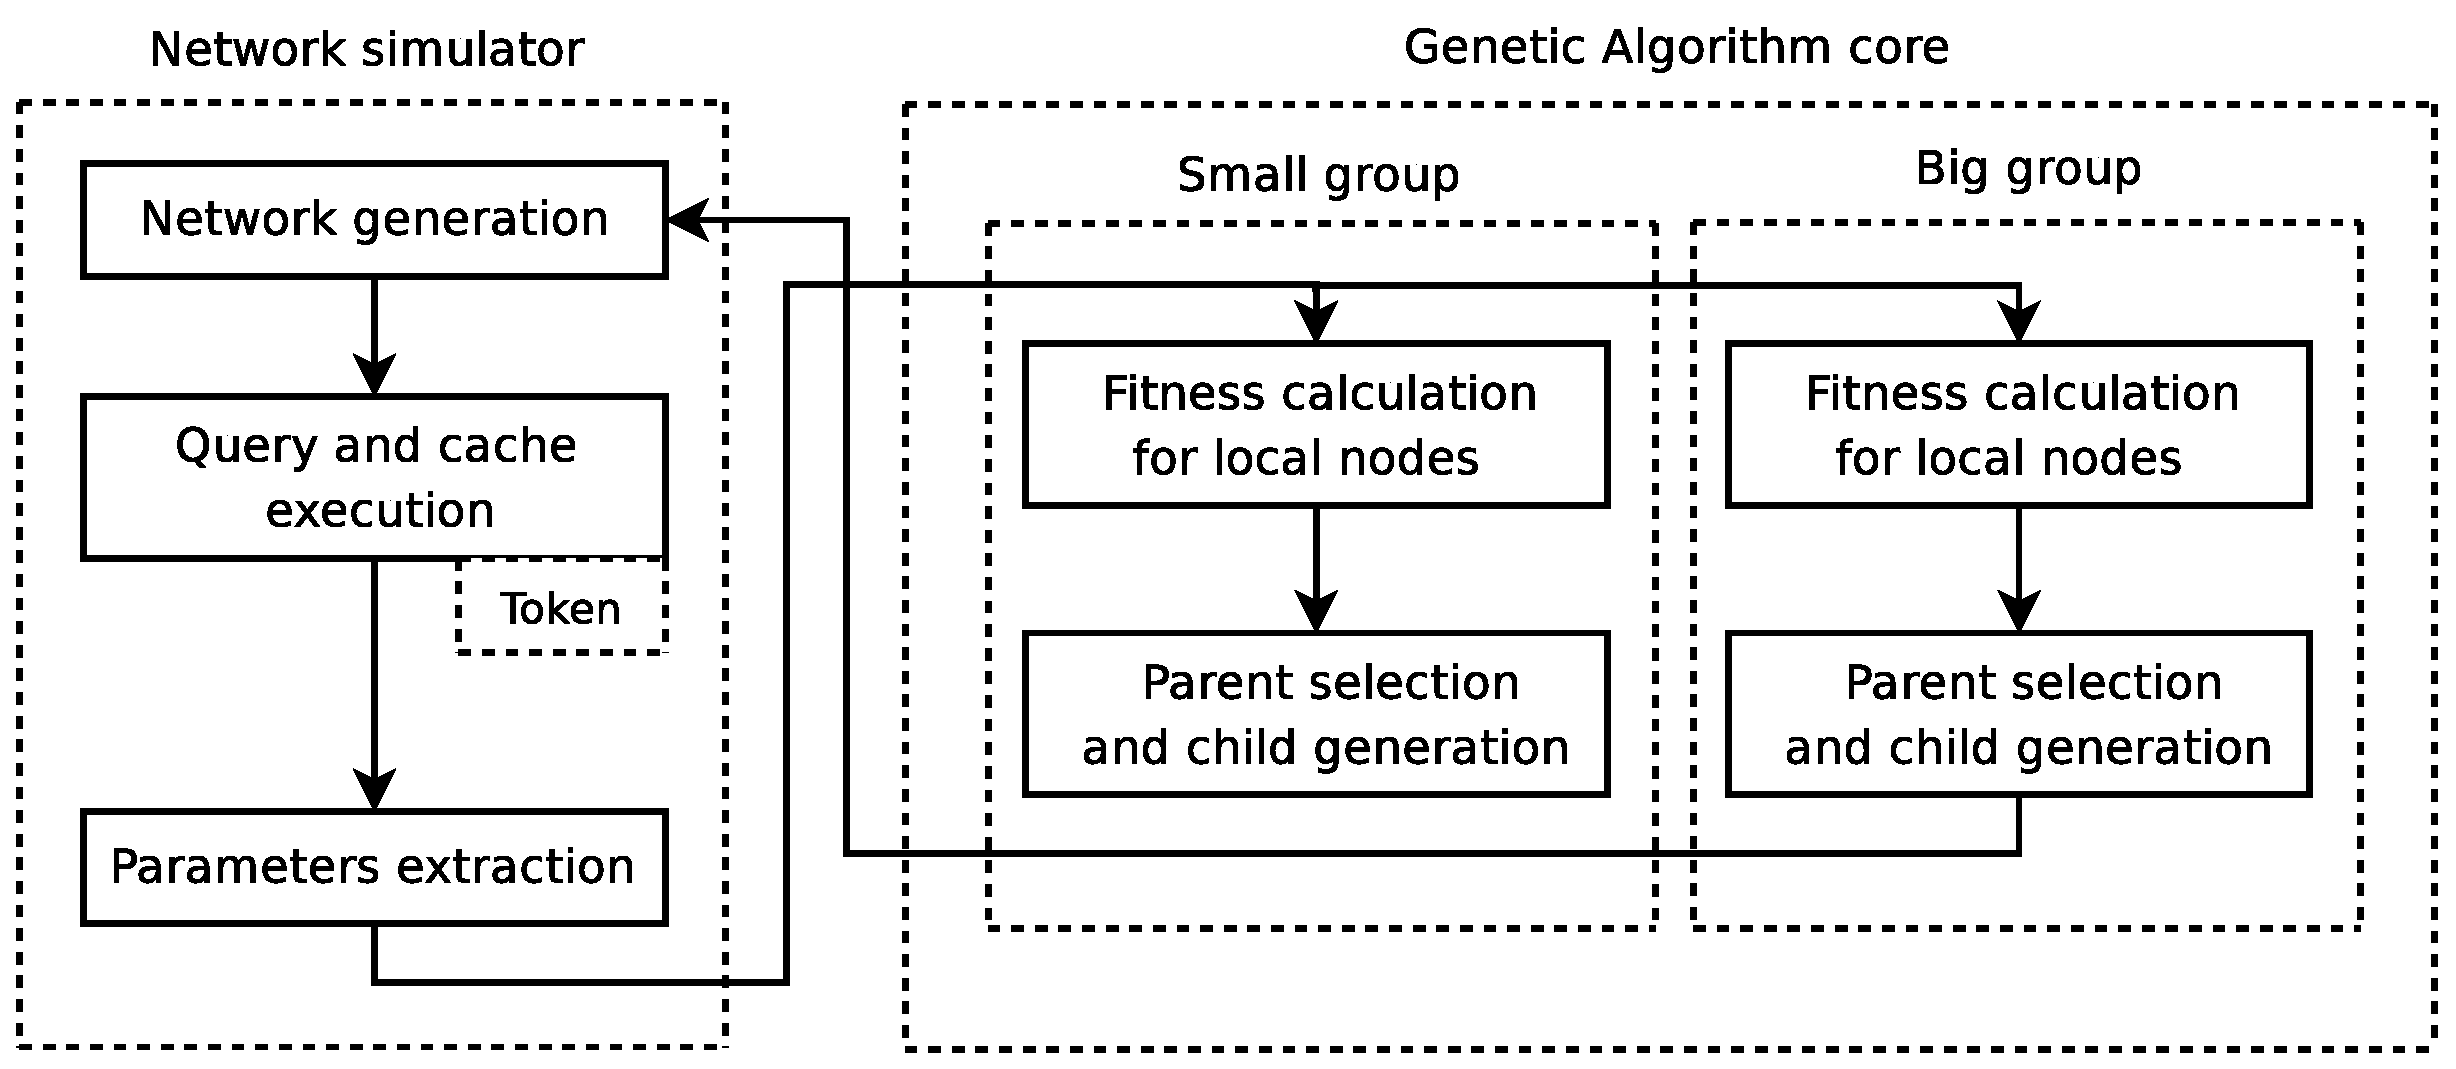
\includegraphics[width=5.2in]{simblock}
\caption{Block diagram for Genetic algorith simulator} 
\label{fig:simblock}
\end{figure}

\subsection{Network model}\label{sec:netmodel}
Figure \ref{fig:network} shows our model for the unstructured p2p network for file sharing with
$N$ nodes. To construct the network model, we use $netmodeler$ which is C++ library for
modeling networks developed at University of Florida and UCLA\cite{netmodeler}.

\begin{figure}
\centering
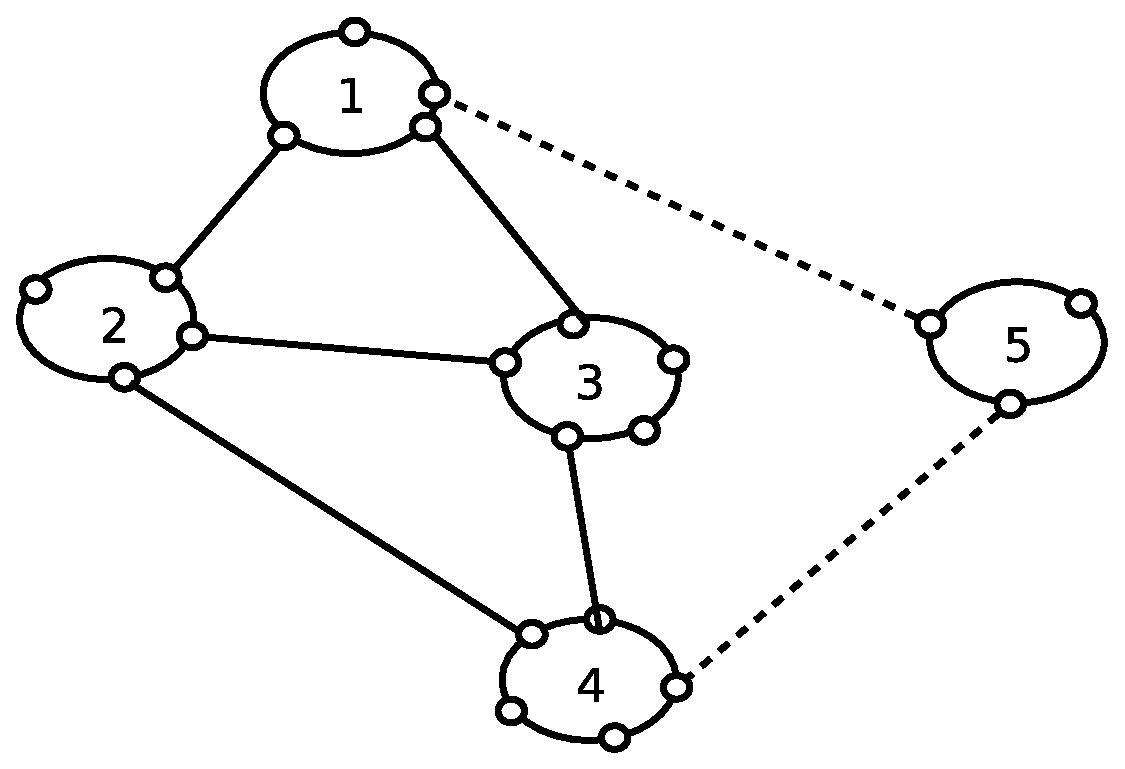
\includegraphics[width=2.5in]{network}
\caption{Network Configuration} 
\label{fig:network}
\end{figure}

Our network model consists of two parts; network configuration and network operation such
as query and cache action. In network configuration period, $N$ nodes sequentially join the
network attaching to two existing nodes randomly selected. At that time, three parameters,
which describe the characteristics of node, are assigned to joining node; message ignore
probability, TTL and connection limit. Firstly, message ignore probability reflects the
selfishness of users. In other words, nodes, which have high message ignore probability, tend
to seldom responses any query and cache actions from its neighbors. Message ignore
probability is assigned to node with uniformly distributed probability. TTL and connection
limit are selected within bounded range and assigned to new generated node. In figure 2,
marks around nodes mean the number of connection limit to be able to connect to neighbors.
Also, if new joining node asks to connect to full-connected node, the request is denied and re-
asked to another node.

After network configuration is completed, each node executes cache and query actions as
following: The node $n_A$ has a certain character string $I_A$ as item. This character string is
generated by \emph{randomstringgenerator}. For system stabilization, the node $n_A$ replicates its own
item to neighbors with broadcast whose size depends on the value of TTL and connection
limit. Followed by cache for $I_A$, another node, $n_B$, randomly selected requests the query for
item $I_A$ to its neighbors. For adequate result acquisition, we ran 100 query actions per a cache
action with different request nodes.

In order to evaluate the network performance, we refer to communication traffic and
memory consumption as CPU and disk cost. Also, we identify the benefit which node
attempts to maximize as hitrate. Hitrate, CPU and disk cost are defined by
\[
Hitrate=\frac{Query_{resp}}{Query_{req}}
\]
\[
CPU\_cost=Message_{recv}+Message_{proc} \times N_{items}
\]
\[
disk\_cost=N_{items}
\]

where $Query_{req}$ and $Query_{resp}$ refer to the number of queries that 
the node requests and is answered by neighbors repectively. $Message_{recv}$ and $Message_{proc}$ 
represent the number of messages that the node received and processed. 
Also, $N_{items}$ is the number of items that the node obtains.

\subsection{Genetic algorithm}\label{sec:genetic}
Since local nodes tend to minimize its own loads such as communication traffic and memory
consumption, but maximize the number of hits which gets for its queries, cheating strategy of
free riders is able to arise naturally. For these reasons, we apply the genetic algorithm to
observe the intention and behavior of local nodes. In fact, our key idea is derived from the
concept of the GA which finds the optimal parameters to maximize the fitness. To do this,
each node in the network is regarded as individual which organizes one generation and the
node characteristics parameters –message ignore probability, TTL, and connection limit – are
considered as gene for each individual.
Also we established the fitness function using parameters defined in previous section: Hitrate,
CPU and disk cost. The fitness function evaluates the quality of individuals and is used to
select parents nodes.
\[
Fitness = Exp\{\alpha_{h}\times hitrate-(\alpha_{c}\times cpu_cost + \alpha_{d}\times disk_cost)\}
\]

where $\alpha$ is normalization factor. We distinguished the fitness function with positive and
negative part. Positive part includes the hitrate and negative part consists of the CPU and disk
cost. Therefore, as CPU and disk cost decrease and hitrate increases, fitness will increase.
After network operation process, each node estimates its own hitrate, CPU and disk cost and
the GA core calculates the fitness of each node. Fitness obtained by fitness function is used to
rank nodes for parent selection. Based on the ranked nodes, GA core selects parent nodes and
generates child nodes by crossover and mutation operation of three genes of parents ;
message ignore probability, TTL and connection limit. The crossover and mutation of each
gene is following as:\\

\begin{itemize}
\item{\bf Message ignore probability -}
$Average[Father, Mother] + m\% of mutation$
\item{\bf TTL -}
$Random[Father, Mother] + t\% of mutation$
\item{\bf Connection limit -}
$Random[Father, Mother] + c\% of mutation$\\
\end{itemize}

For our simulation, we set 5\%, 0.1\% and 0.1\% for mutation of Message ignore probability,
TTL and connection limit respectively. Because the values of TTL and connection limit are
positive integer and bigger than message ignore probability, we set relatively small value for
the mutation of TTL and connection limit over message ignore probability. In parent selection
process, we have tried several methods to reduce the computation loads of genetic algorithm.
As a result, we decided the square-root selection method\cite{genetic}. In addition, allowing any pair of
nodes to mate to produce a child keeps all the nodes mixing together. It prevents the natural
evolution of free riders. For that reason, we make two populations, the big group and small
group. Mating only happens in the same group: both of parents, father and mother, need to be
from the same group. Actually, in our setting, the ratio of small group and big group is 1 to 9.

\section{Evolution of free riders}\label{sec:evolution}
In this section, we show that free riders can naturally evolve. Firstly, we demonstrate the
intention of free riders in the absence of punishment. Furthermore, against the cheating
strategy of free riders, we introduce the simple solution which stops the free riders taking
benefits from network without any contribution. In practice, making the cheating strategy be
broken by taking some countermeasure, we can stop free riders. The countermeasure we
propose is based on exchanging reciprocal token. In fact, the ability of the node to get the
resource that neighbor possesses depends on the number of reciprocal tokens.

\subsection{The problem of free riders}\label{sec:problem}
The problem of free riders is no contribution but only taking resource from network. 
In this section, we demonstrate the problem of free riders. Figure \ref{fig:nocpucost}, \ref{fig:nodiskcost}, 
\ref{fig:nohitrate}, and \ref{fig:fitness1} show hitrate, CPU / disk cost and fitness value
for given message ignore probability without any punishment on free riders. In contrast with
CPU and disk cost which are internally related to its own characteristics, p\_ignore, hit rate is
external factor affected by response of neighbors. Actually, in figure \ref{fig:nocpucost} and \ref{fig:nodiskcost}, 
it can show that CPU and disk cost decrease, as message ignore probability, \emph{p\_ignore}, increases. Because
the nodes which have high message ignore probability process fewer cache and query
messages, they have smaller CPU and disk cost than low ignore probability nodes. However, in
figure \ref{fig:nohitrate}, it is shown that the distribution of hit rate is unrelated to message ignore
probability. Totally, as shown in figure \ref{fig:fitness1}, in case of fitness value which is calculated using
message ignore probability, CPU and disk cost, fitness value increases as message ignore
probability increases.

\begin{center}
\begin{figure*}[ht]
\centering
\begin{tabular}{c c}
\begin{minipage}[t]{3in}
\centering
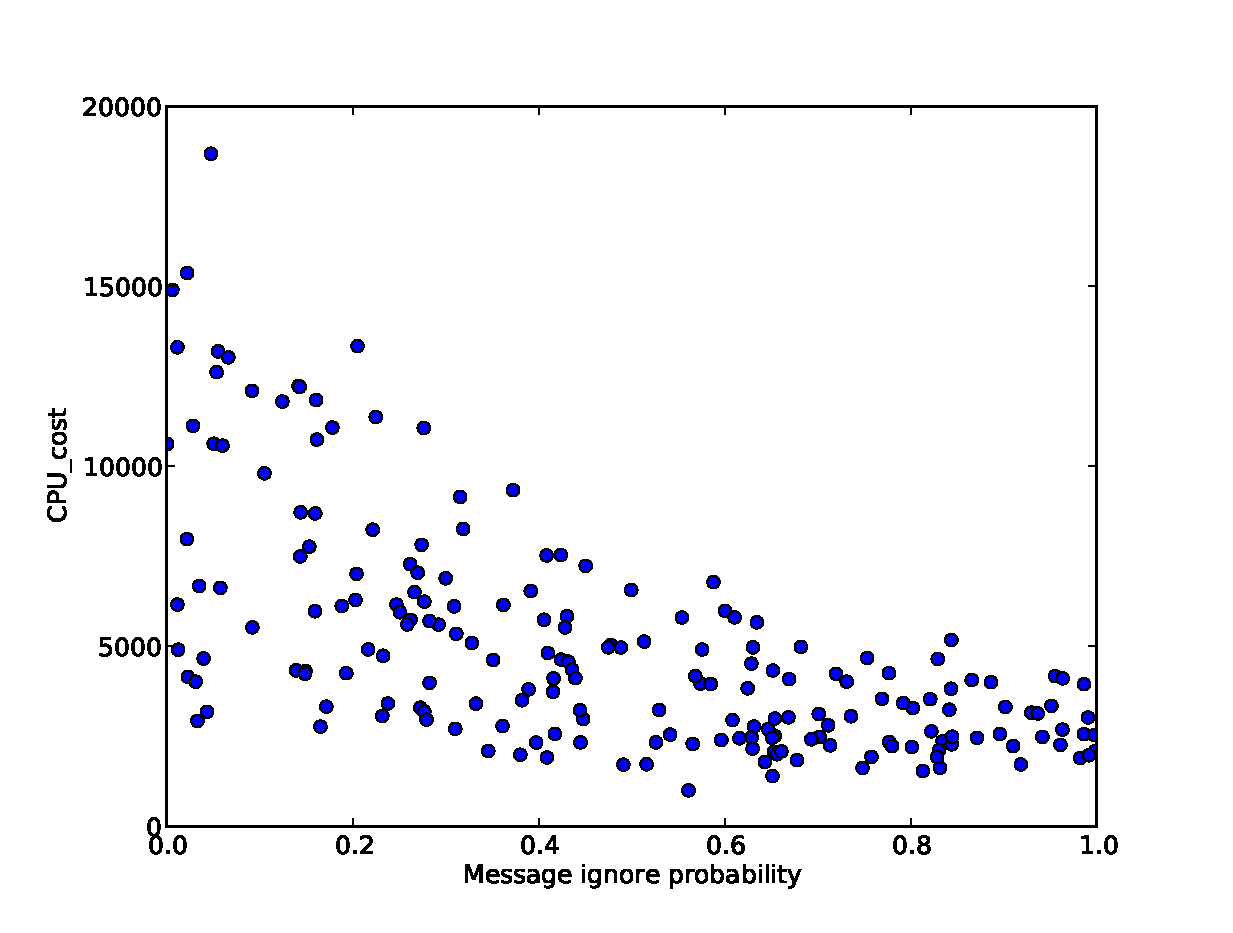
\includegraphics[width=3in]{cpucost1}
\caption{CPU\_cost for message ignore probability}
\label{fig:nocpucost}
\end{minipage}
\begin{minipage}[t]{3in}
\centering
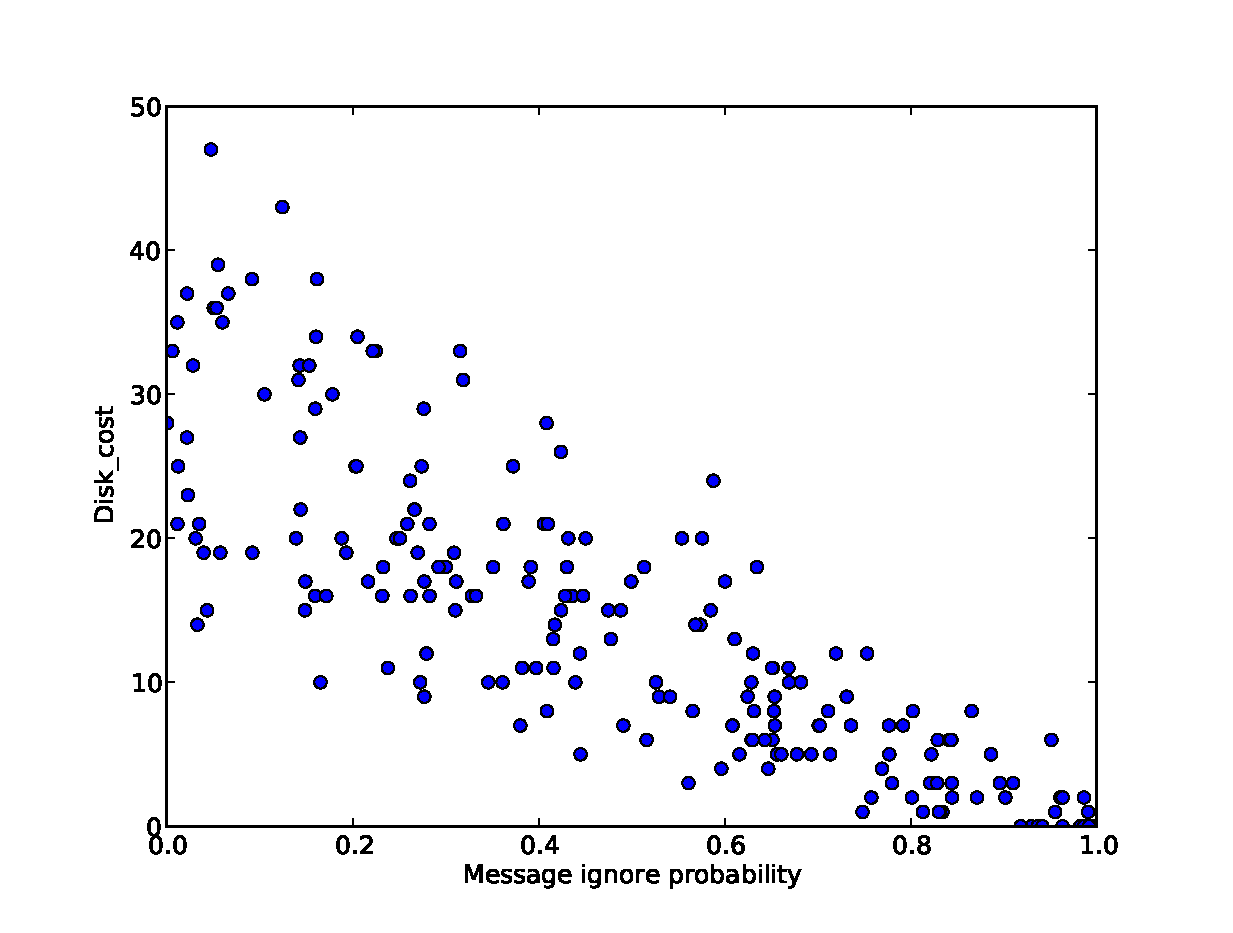
\includegraphics[width=3in]{diskcost1}
\label{fig:nodiskcost}
\caption{Disk\_cost for message ignore probability}
\end{minipage}
\end{tabular}
\end{figure*}
\end{center}

\begin{center}
\begin{figure*}[ht]
\centering
\begin{tabular}{c c}
\begin{minipage}[t]{3in}
\centering
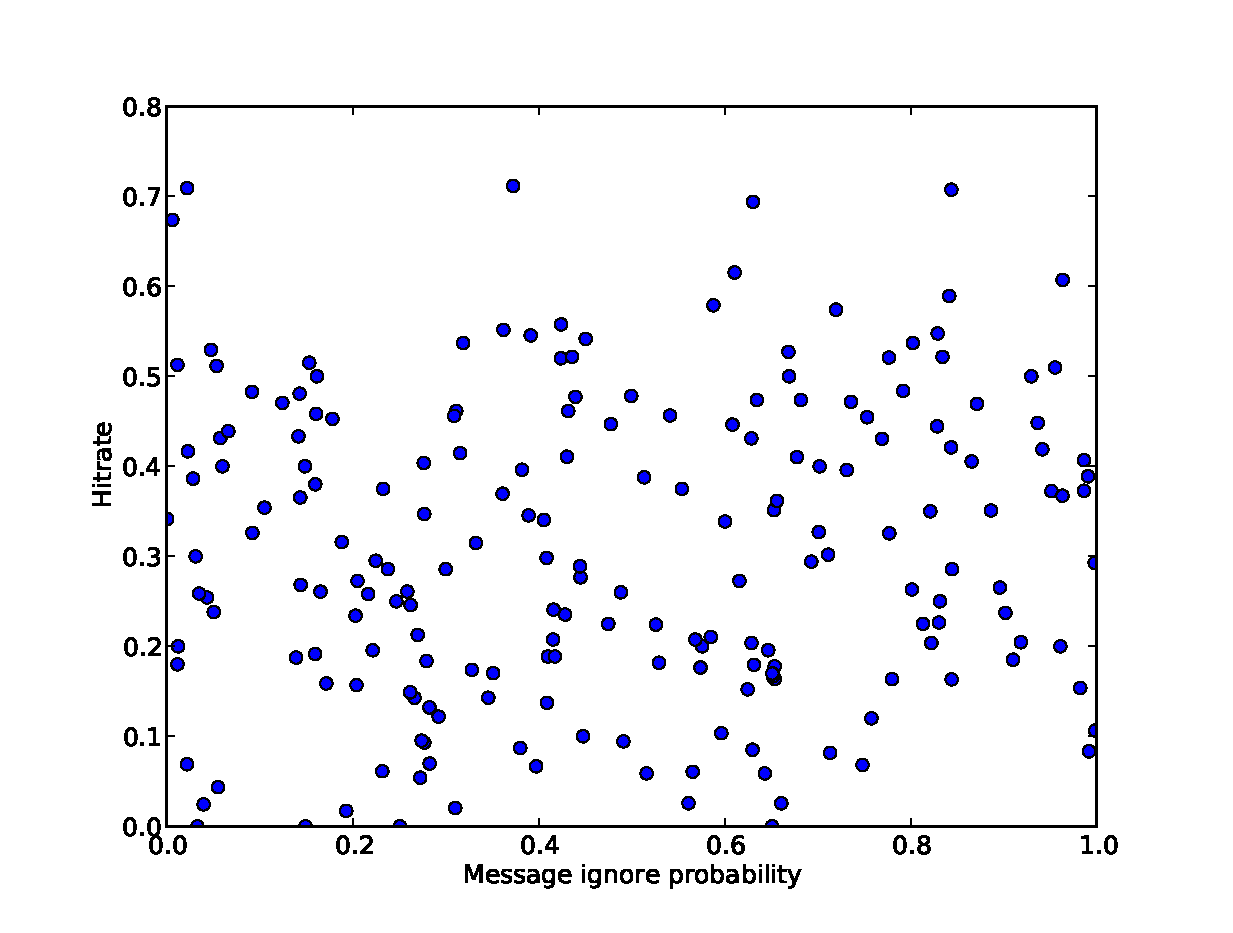
\includegraphics[width=3in]{hitrate1}
\caption{Hitrate for message ignore probability}
\label{fig:nohitrate}
\end{minipage}
\begin{minipage}[t]{3in}
\centering
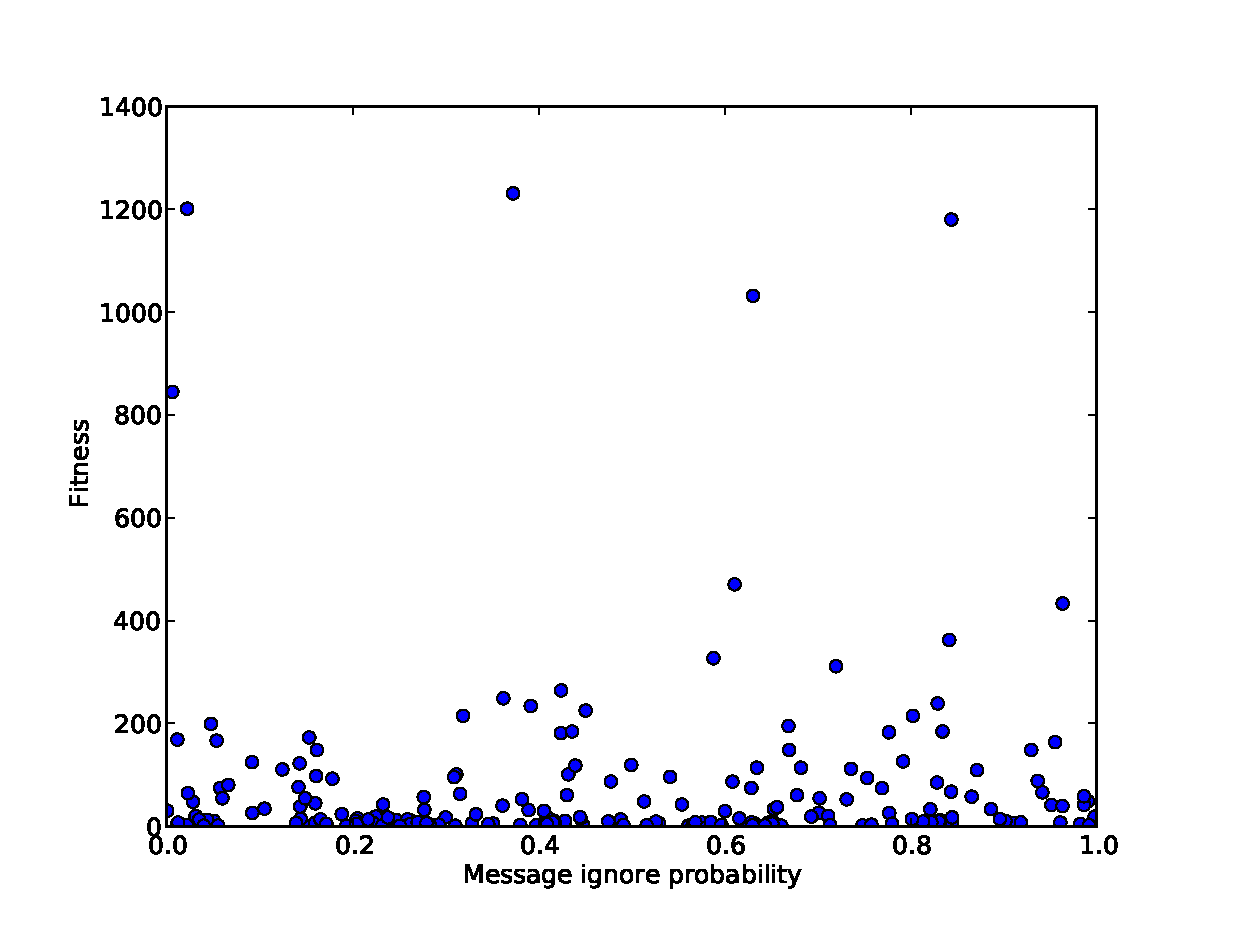
\includegraphics[width=3in]{fitness1}
\label{fig:fitness1}
\caption{Fitness for message ignore probability}
\end{minipage}
\end{tabular}
\end{figure*}
\end{center}

The evolution of message ignore probability, hitrate, CPU and disk cost over generations are
illustrated in figure \ref{fig:noprob}, \ref{fig:nohit}, \ref{fig:nocpu}, and \ref{fig:nodisk}. 
In figure \ref{fig:noprob}, small group allowed to evolve independently becomes selfish, 
which maintain high message ignore probability. This is because increasing
message ignore probability saves CPU and disk cost but does not hurt its hitrate. In fact,
figure \ref{fig:nohit} shows that hitrate of small group is almost identical to that of big group. However,
in case of CPU and disk cost, small group has an extremely slight CPU and disk cost. In next
section, we simulate the identical situation to this section except for applying the
countermeasure and present different evolution pattern of free riders.

\begin{center}
\begin{figure*}[ht]
\centering
\begin{tabular}{c c}
\begin{minipage}[t]{3in}
\centering
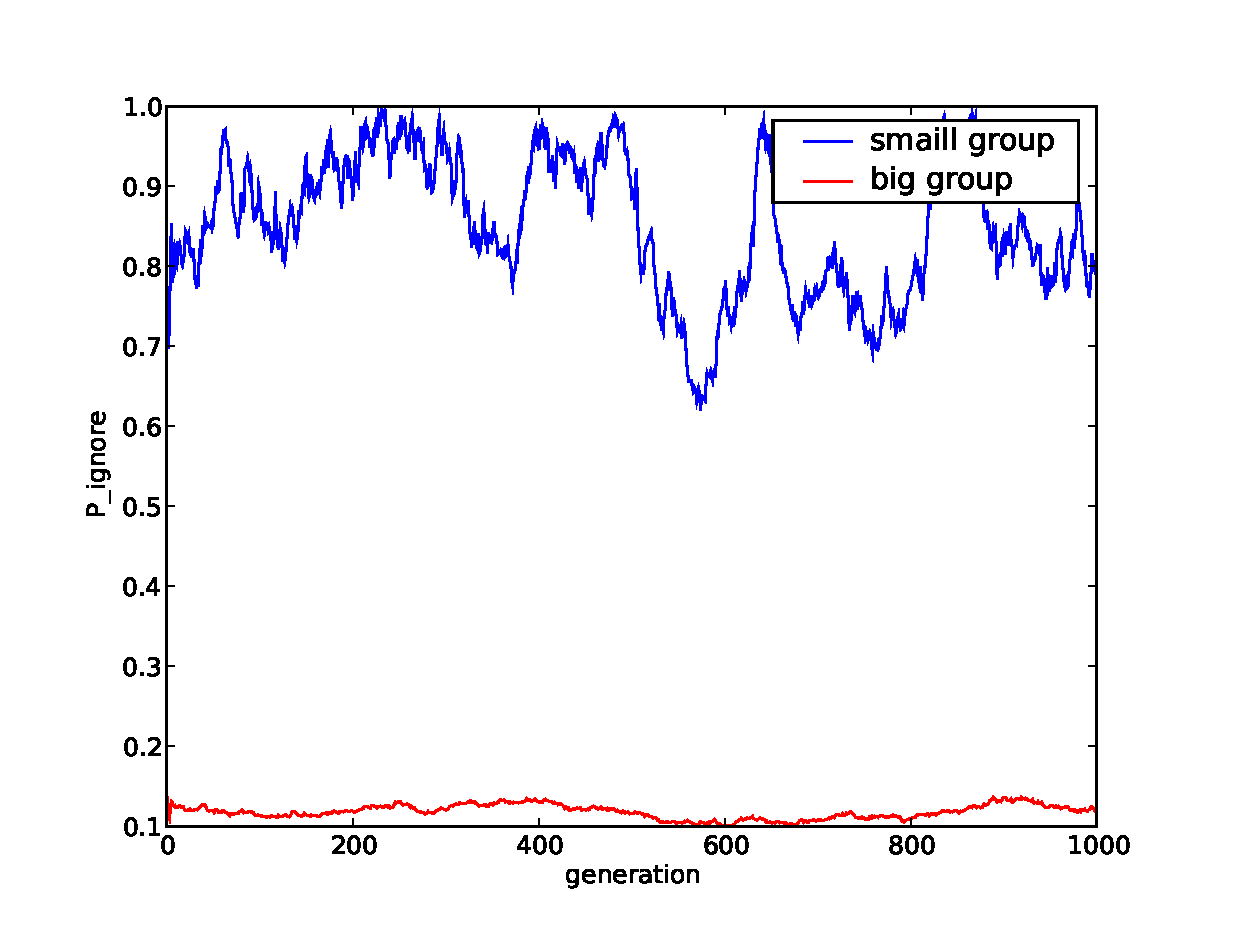
\includegraphics[width=3in]{notokenprob}
\caption{The evolution of message ignore probability without any contermeasure}
\label{fig:noprob}
\end{minipage}
&\begin{minipage}[t]{3in}
\centering
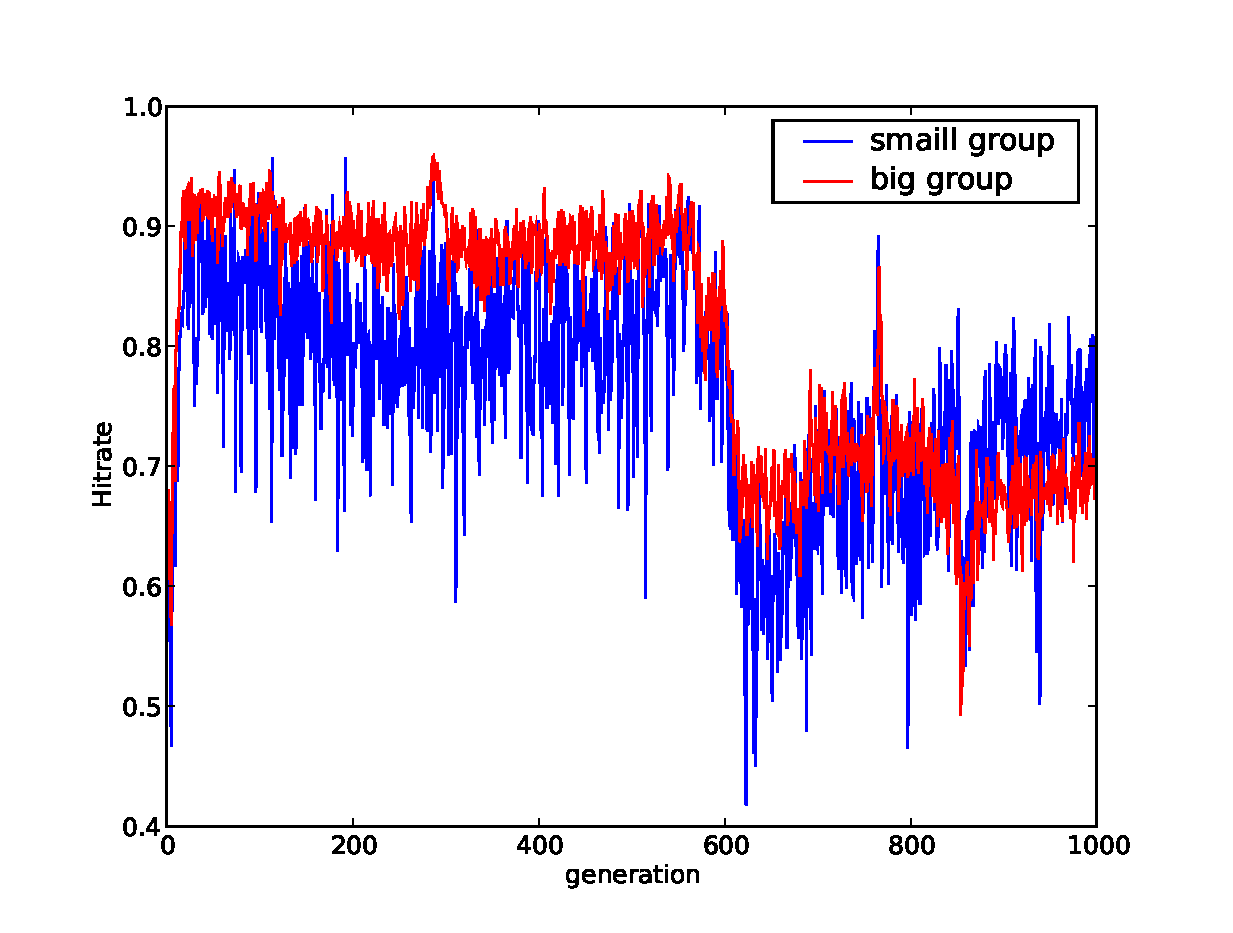
\includegraphics[width=3in]{notokenhit}
\label{fig:nohit}
\caption{The evolution of hitrate without any contermeasure}
\end{minipage}
\end{tabular}
\end{figure*}
\end{center}

\begin{center}
\begin{figure*}[ht]
\centering
\begin{tabular}{c c}
\begin{minipage}[t]{3in}
\centering
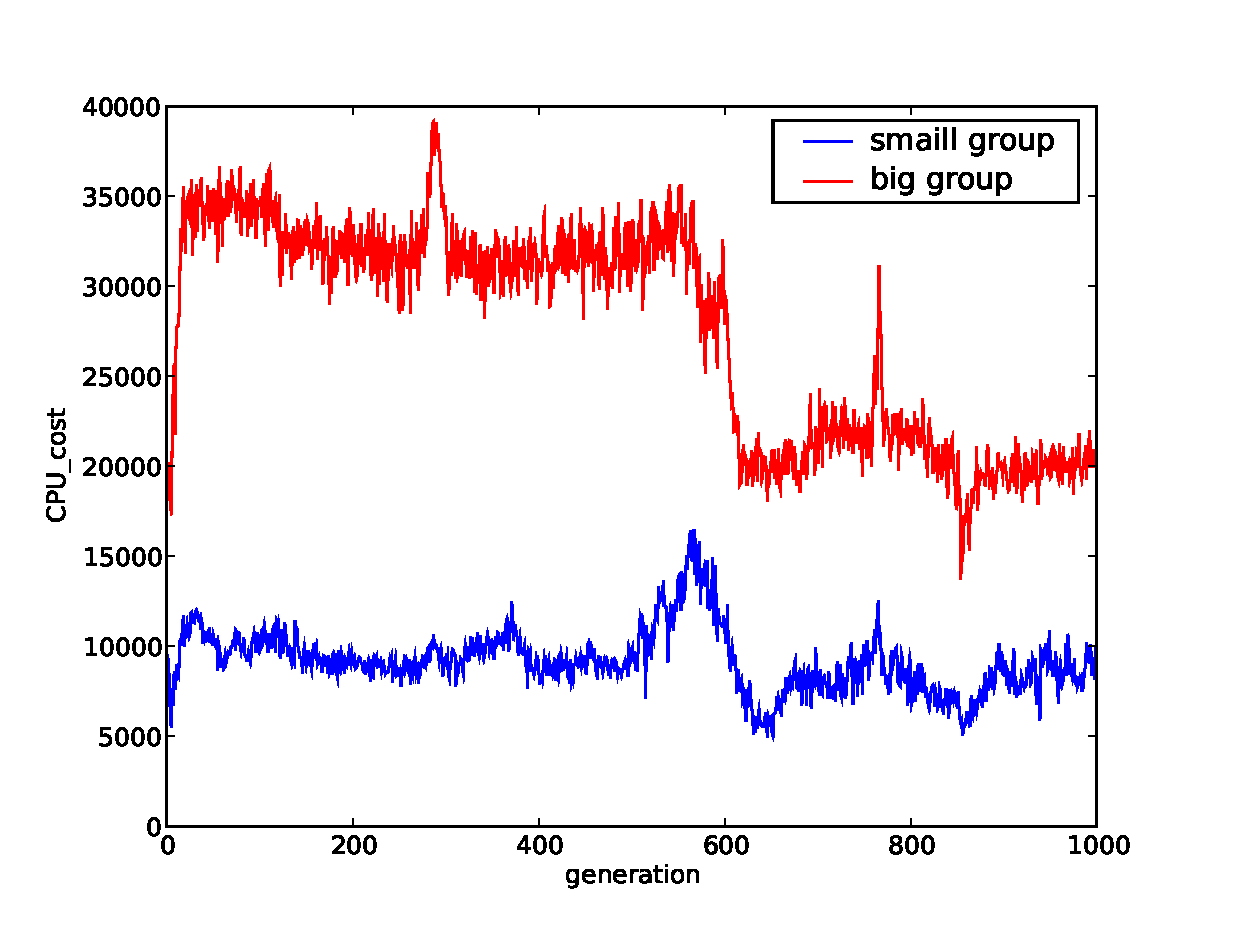
\includegraphics[width=3in]{notokencpu}
\caption{The evolution of CPU\_cost without any countermeasure}
\label{fig:nocpu}
\end{minipage}
&\begin{minipage}[t]{3in}
\centering
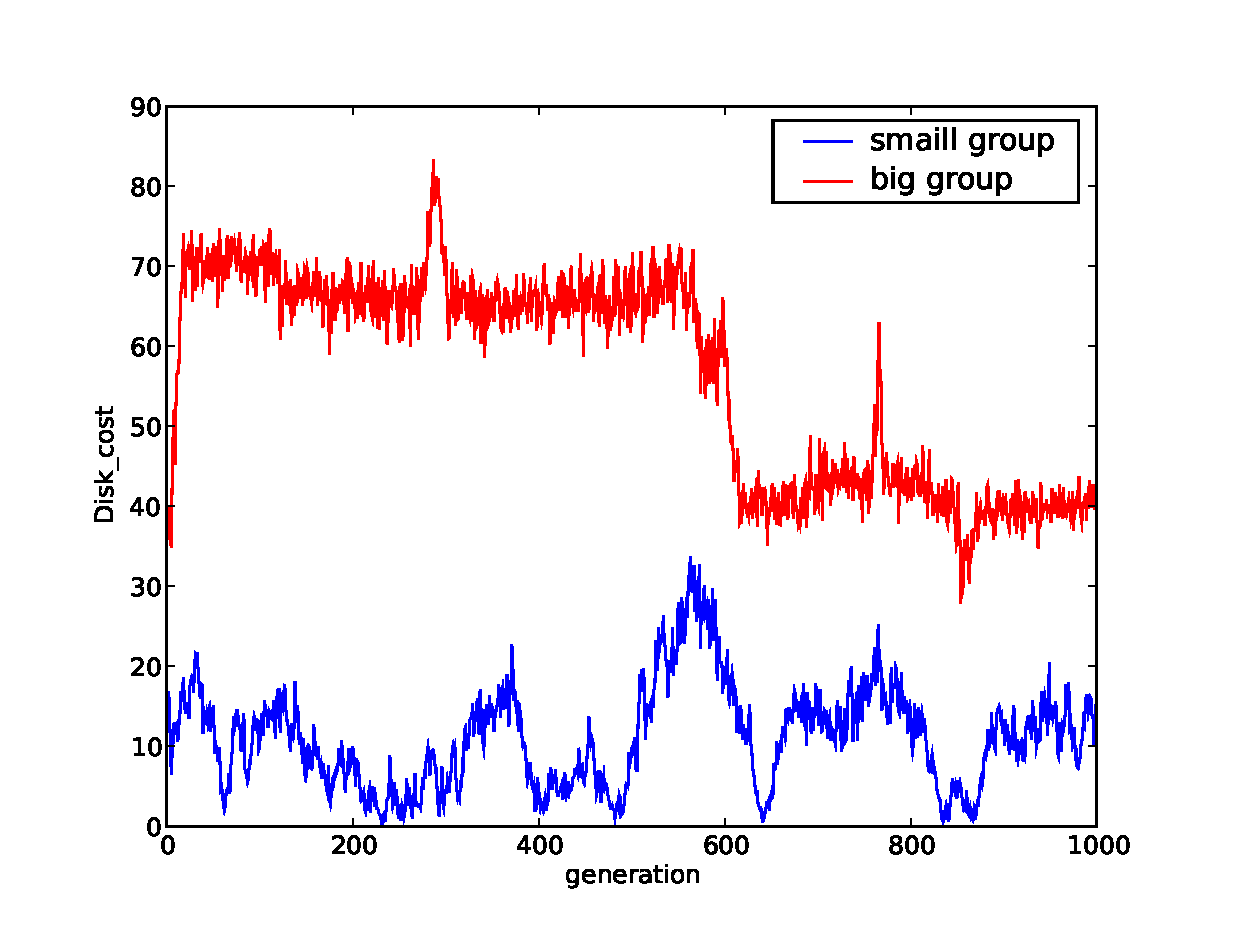
\includegraphics[width=3in]{notokendisk}
\label{fig:nodisk}
\caption{The evolution of disk\_cost without any countermeasure}
\end{minipage}
\end{tabular}
\end{figure*}
\end{center}

\subsection{Countermeasure}\label{sec:countermeasure}
Our goal is to punish the hit rate of nodes with high message ignore probability. 
It is alsoexpected that this punishment makes free riders relieve its selfishness. To implement the
punishment, we propose the reciprocal token method where node‟s capability to take items is
based on the number of token. In this method, each node in the network maintains the
neighbor token table which contains token information of its own neighbor. The token
information consists of the address of neighbors and its tokens for neighbors. Initially, in
node joining process, the node connected to existing node pushes the address of existing node
and initial token values into an empty entry of neighbor token table. Such initial token value
is to give the chance which can contribute to the network so that each node earns token
enough to share network resource. To help understand of the token method, we describe three
scenarios as shown in figure 1. The node $n_A$, sends a query to connected node $n_B$, $n_C$ and
disconnected node $n_D$. (The region of query) In first scenario, $n_B$ searches its neighbor token
table and serves required item if tokens for $n_A$ remain. As the consideration for $n_B$'s sharing,
$n_A$ increases the tokens for nB by one. On the other hands, $n_B$ decreases the tokens for $n_A$ by
one. Secondly, if $n_C$ ignore the query of $n_A$ or do not have the requested item, $n_A$ updates its
own neighbor token table decreasing the token for $n_C$. For last case, we consider the
disconnection between request and requested node. First of all, $n_D$ which have no information
about request node, $n_A$ creates the entry for $n_A$ and initiates token value. Also node $n_A$
appends the information for $n_D$ into the neighbor token table and decreases the $n_D$'s tokens
because $n_D$ ignores the query.

\begin{figure}
\centering
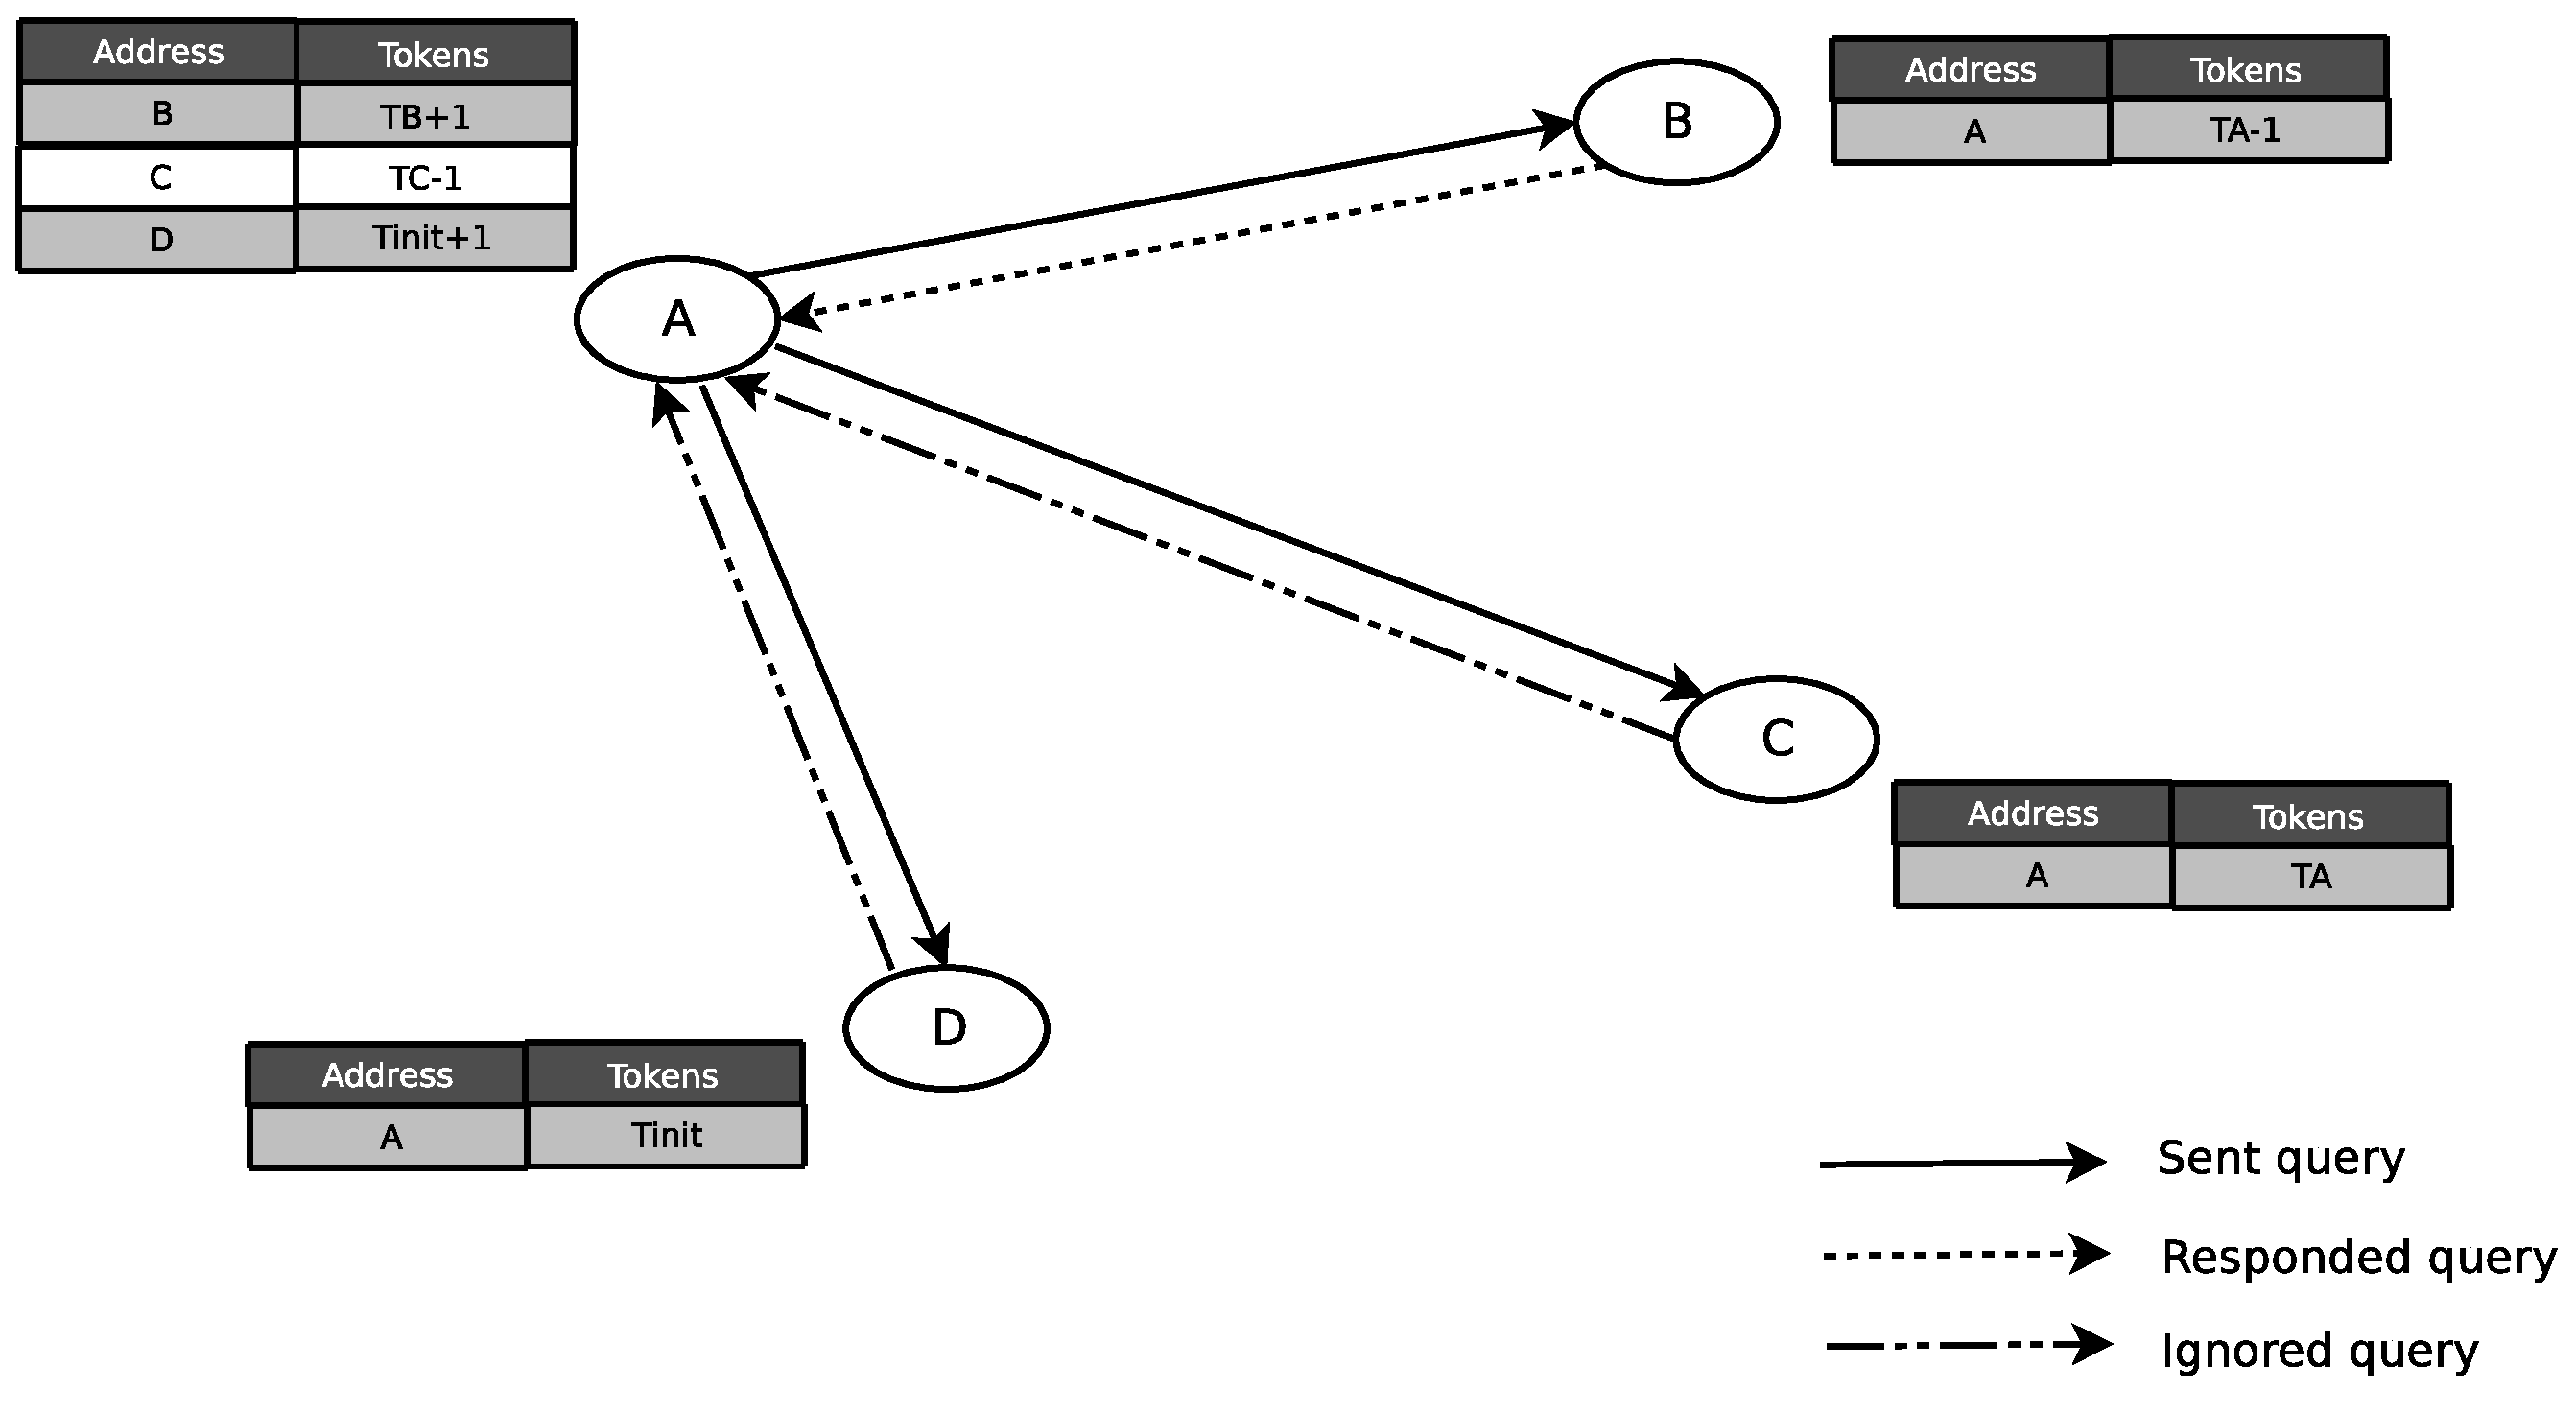
\includegraphics[width=5in]{token}
\caption{Reciprocal token method} 
\label{fig:token}
\end{figure}

In reciprocal token method, the nodes which intentionally ignore the queries of neighbors
with high message ignore probability exhaust its tokens, and eventually, cannot take any
advantages from the network. Ultimately, the nodes have to relieve their selfishness to get the
benefits. Our protocol is very simple, but it is enough to lead for free riders to contribute to
the network.

\begin{figure}
\centering
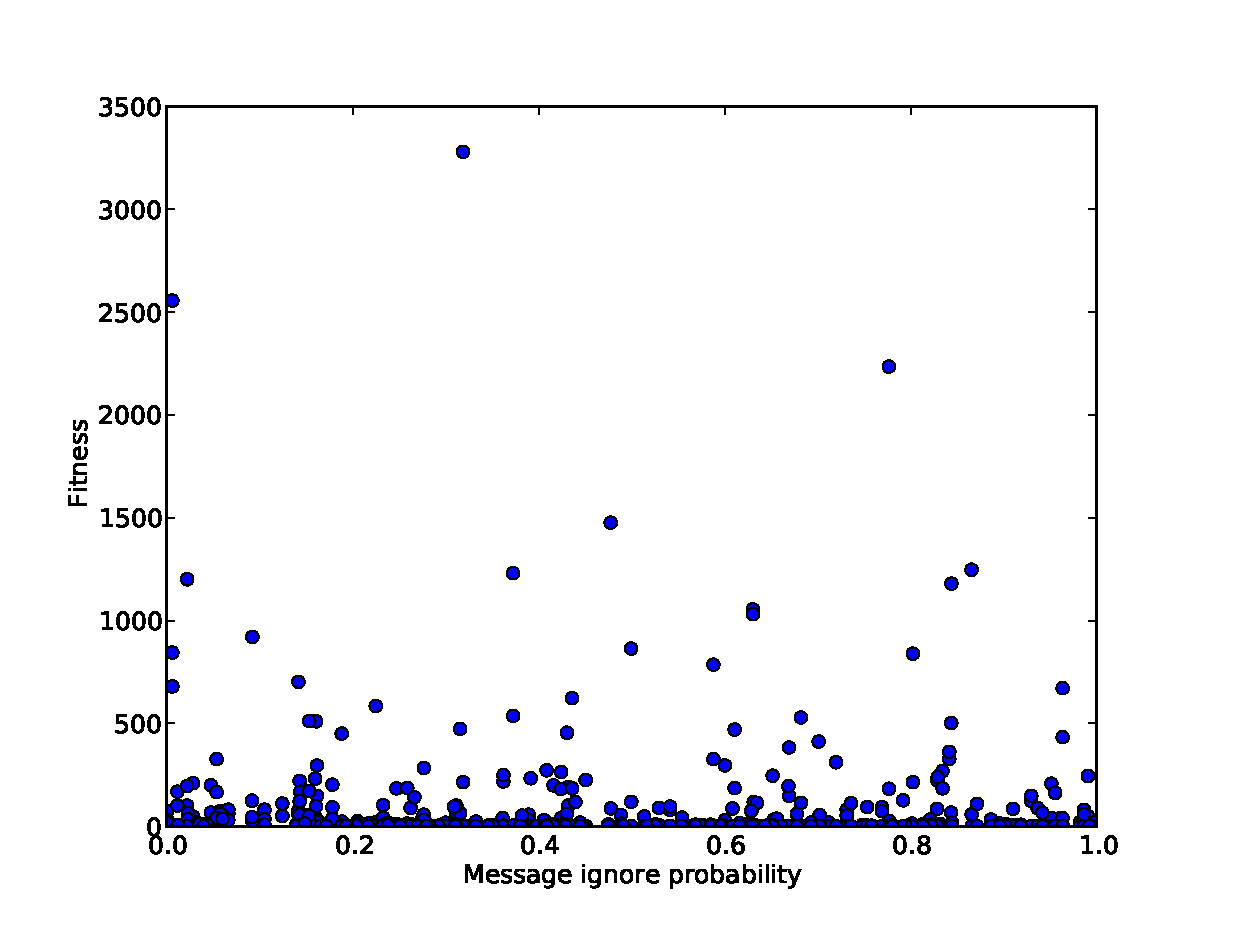
\includegraphics[width=3in]{fitness2}
\caption{Fitness value for message ignore probability with reciprocal token method}
\label{fig:tokenfit}
\end{figure}

\begin{center}
\begin{figure*}[ht]
\centering
\begin{tabular}{c c}
\begin{minipage}[t]{3in}
\centering
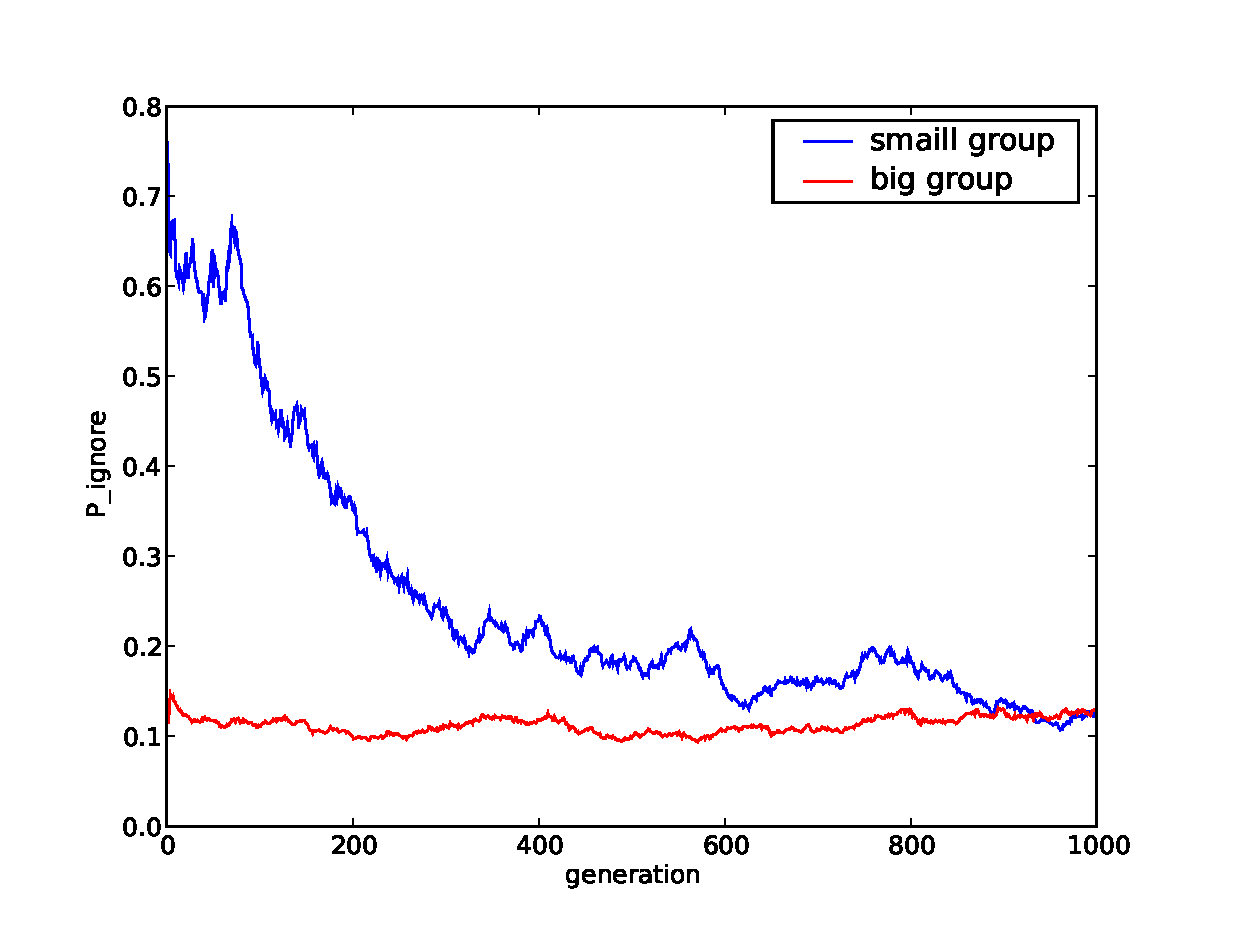
\includegraphics[width=3in]{tokenprob}
\caption{The evolution of message ignore probability with reciprocal token method as generation goes on}
\label{fig:tokenprob}
\end{minipage}
&\begin{minipage}[t]{3in}
\centering
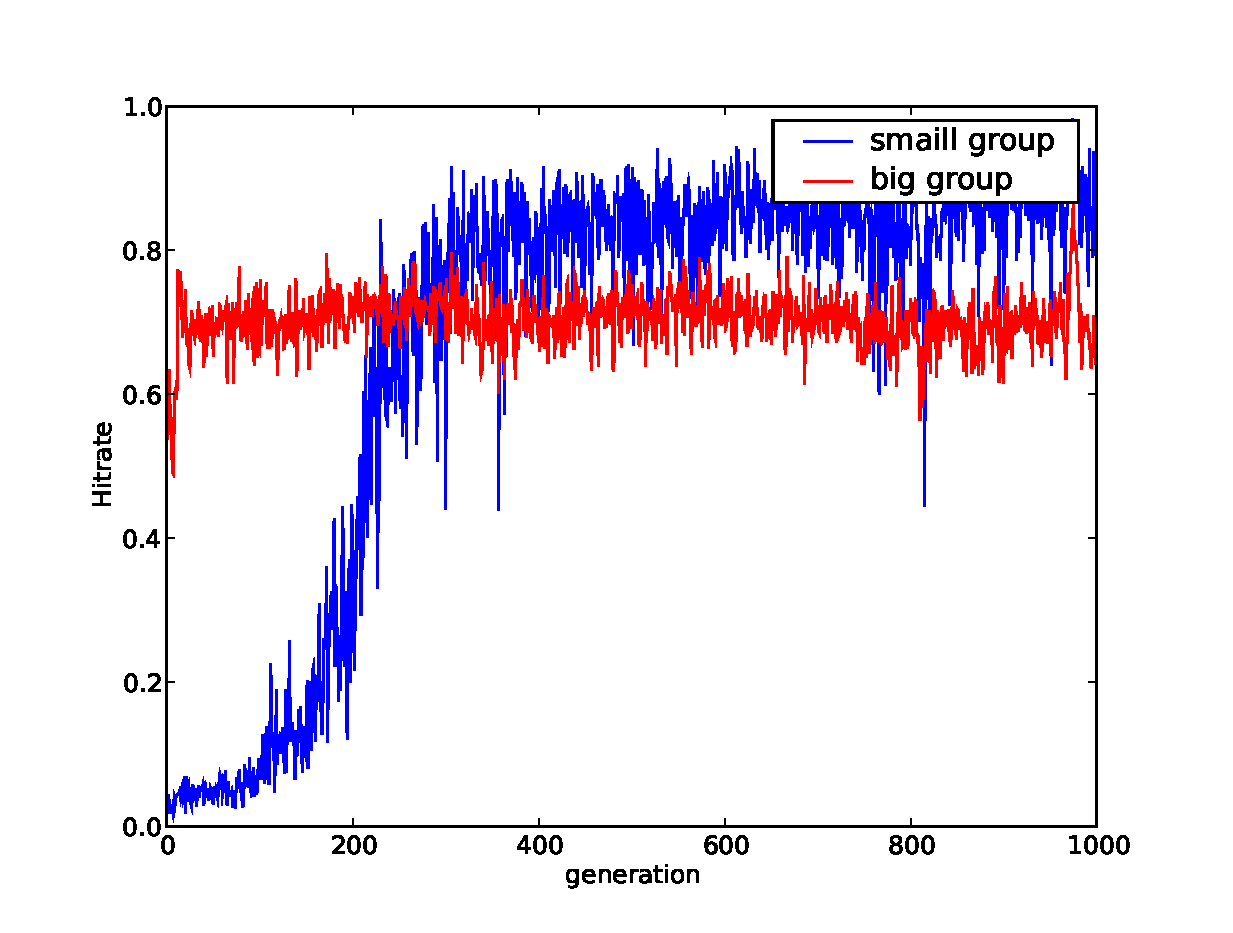
\includegraphics[width=3in]{tokenhit}
\caption{The evolution of hitrate with reciprocal token method as generation goes on}
\label{fig:tokenhit}
\end{minipage}
\end{tabular}
\end{figure*}
\end{center}

\begin{center}
\begin{figure*}[ht]
\centering
\begin{tabular}{c c}
\begin{minipage}[t]{3in}
\centering
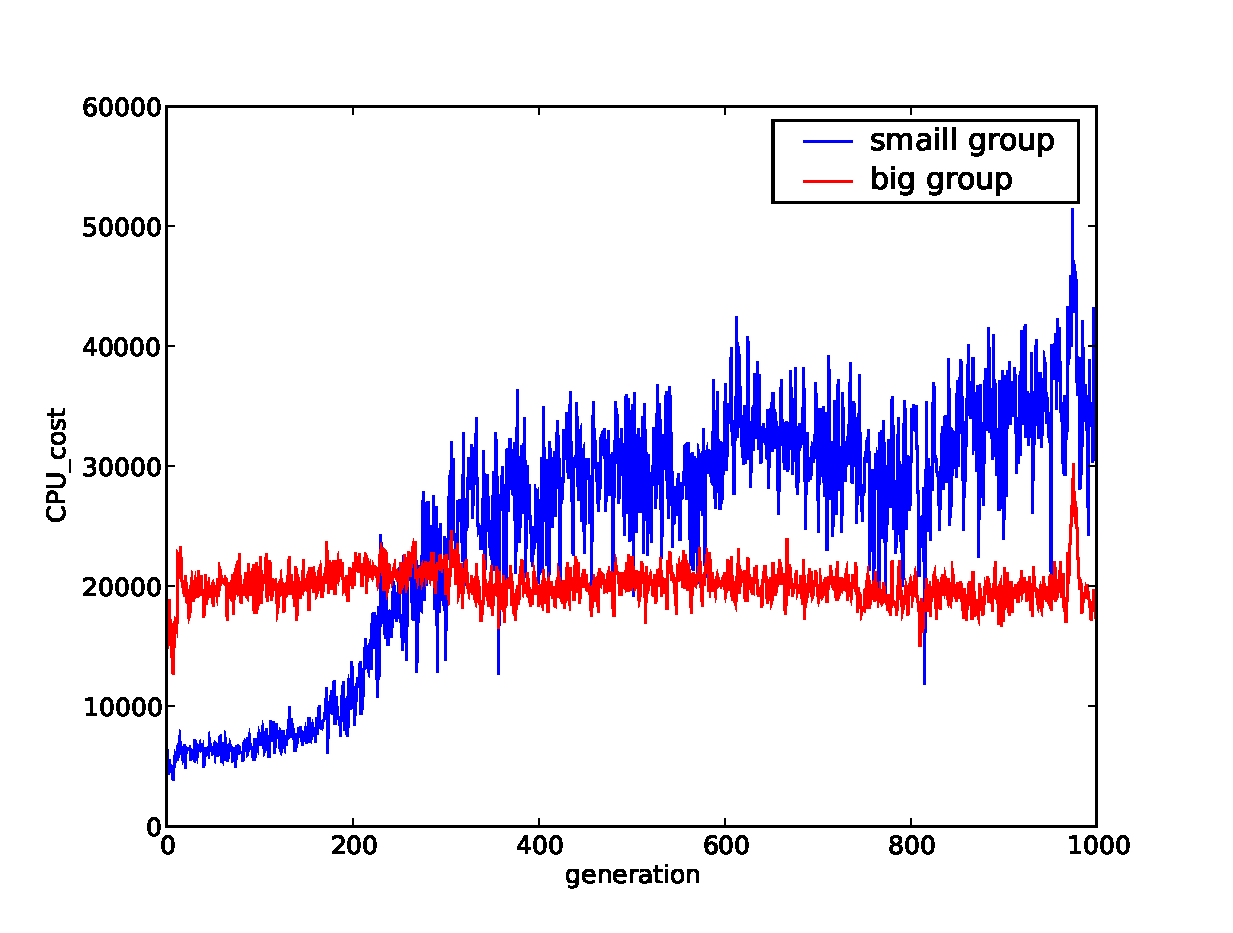
\includegraphics[width=3in]{tokencpu}
\caption{The evolution of CPU\_cost with reciprocal token method as generation goes on}
\label{fig:tokencpu}
\end{minipage}
&\begin{minipage}[t]{3in}
\centering
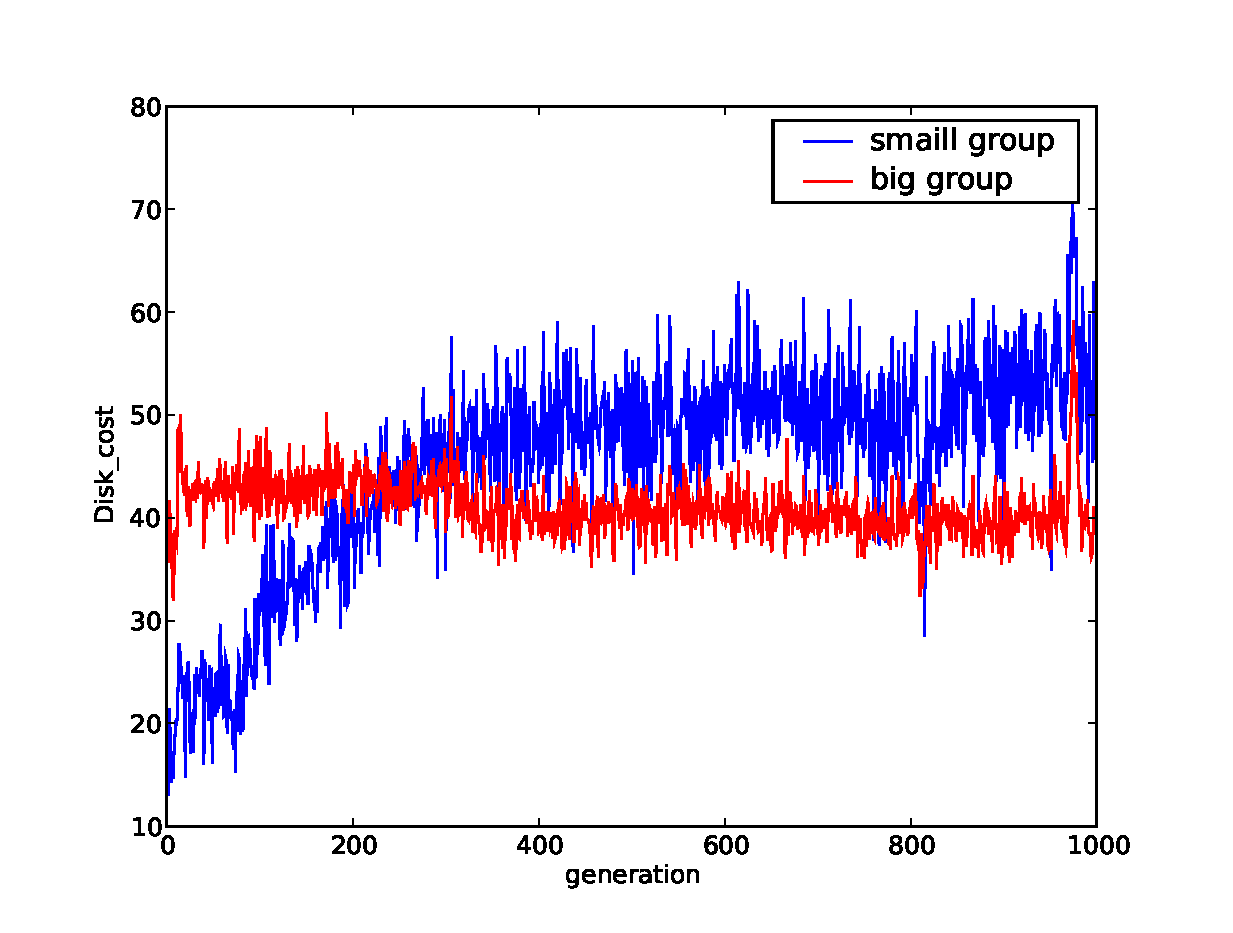
\includegraphics[width=3in]{tokendisk}
\caption{The evolution of disk\_cost with reciprocal token method as generation goes on}
\label{fig:tokendisk}
\end{minipage}
\end{tabular}
\end{figure*}
\end{center}


Figure \ref{fig:tokenfit}, \ref{fig:tokenprob}, \ref{fig:tokenhit}, \ref{fig:tokencpu}, and \ref{fig:tokendisk}
show the evolution of free riders with reciprocal token method over generations.
Firstly, figure \ref{fig:tokenfit} displays the fitness value while applying the token method. 
The fitness value decreases as message ignore probability increases. It means that the node which have
high message ignore probability cannot take any benefits from network. Also, in figure \ref{fig:tokenprob}
and \ref{fig:tokenhit}, hitrate of small group in early generation is almost 0 due to high message ignore
probability. However, as generation goes on, small group decreases its own message ignore
probability in order not to be punished in the network and eventually behaves like big group.
As message ignore probability of small group decreases, hitrate is also similar to big group.

\section{Related Works}\label{sec:related}

Through this paper, we show the natural evolution of free-riding by use of a genetic
algorithm. In fact, applying the genetic algorithm on solving the problem of peer-to-peer
networks has been achieved in various studies. One example of the application of genetic
algorithm to peer to peer networks is to search optimal routing strategy for query and cache.
Firstly, to resolve high bandwidth consumption and poor semi-parallel search, a novel routing
function called \emph{GAroute} is proposed in [1]. In this paper, ID of each peer regards as a gene
and a chromosome which contains a sequence of genes represents a query routing path. In
selection process for next generation, good chromosomes with the highest information gain
and maximum length are primarily selected. Iles et al.[2] explore the search scheme for
routing strategy in peer to peer network using genetic programming. In this study, results
from simulation on peer to peer network are described, in which genetic programming is used
to evolve routing strategies that optimize resource location in various traffic low scenarios.
Network protocol consists of two expressions: the CONN expression which specify the
number of connection to be maintained, and the RANK expression which is used to rank the
connections. Each expression are represented as trees and manipulated using crossover and
mutation operations.
Koo et al.[3] propose a genetic algorithm based neighbor selection strategy which is
incentive-compatible and suitable for real time deployment for peer to peer networks.
Furthermore, the strategy proposed by this study has been compared with the existing
strategy using two welfare metrics: system throughput and average downloading time. In [4],
genetic algorithm is used to find the coarsest \emph{GridPeer} resources. Then, through the
transformation the result of genetic algorithm into the pheromone of ant algorithm, more
accurate resources have been discovered using the ant algorithm.
The most difference between above works and our study is what role genetic algorithm can
play in improving system design. While previous studies we mentioned in this section use the
genetic algorithm as solution to search the optimal value for problems they define, we
employed the genetic algorithm on the top of system observation. There is no intervention of
the genetic algorithm over system components. The punishment of free riders is achieved by
adding tit-for-tat behavior in our work.
In practice, a variety of strategies have been proposed to treat free-riding problem. In [5], a
Gnutella-like unstructured P2P network is proposed to employ free riders to serve as indexing
nodes. Kamvar et al.[6] address free-riding problem via scoring system called as EigenTrust
score which is used to measure the relative participation levels of peer in the system. Also,
Dutta et al.[7] focus on tackling the free-rider with a distributed rating system. Their work
provides two different approaches. In first approach, all users act as a jury to rate each other
based on the service it receives from others and store its own result of ratings. In second
approach, each user has a few designated supervisors and rating value is updated by
supervisors.


\section{Conclusion and Future works}\label{sec:concl}

We have described the intention of free riders using genetic algorithm. Our key idea is
derived from the concept of genetic algorithm which finds the optimal parameters to
maximize the fitness. In order to model free riders, we defined message ignore probability
which presents the degree of selfishness.

In addition, we proposed the simple solution to prevent free riders selfishly behaving and
ultimately induce them to contribute to the network. To do so, we established the neighbor
token table which includes the information about neighbor address and the number of tokens.
Based on its query requests, the node increases or decreases the number of tokens for
neighbors.

Our simulation results present that without any punishment, free riders preserve their
selfishness to maximize the benefits without any contribution to the neighbors. Free riders,
however, evolve to have low message ignore probability in the protocol applied token method
we proposed. Finally free riders behaved like another altruistic peer to stay in the network.

For future works, we need to model free riders more detailed, especially, such as short
network join period and often requiring well-liked items. Using it, we will hopefully modify
our protocol so as to overcome more detailed characteristics of free riders. Furthermore, we
wish to optimize global parameters as well as local parameters through genetic algorithm
which simultaneously regards network and node as population.

\bibliographystyle{IEEEtran}
\bibliography{genetic}

\end{document}

]
